
%(BEGIN_QUESTION)
% Copyright 2012, Tony R. Kuphaldt, released under the Creative Commons Attribution License (v 1.0)
% This means you may do almost anything with this work of mine, so long as you give me proper credit

A technician is installing two pressure alarm switches on a new liquid pipeline pumping station.  The station is still being constructed, with the pipeline empty of all liquid and vented to atmosphere.  One switch detects improper high-pressure conditions on the discharge side of the pump, while the other switch detects improper low-pressure conditions on the suction side of the pump:

$$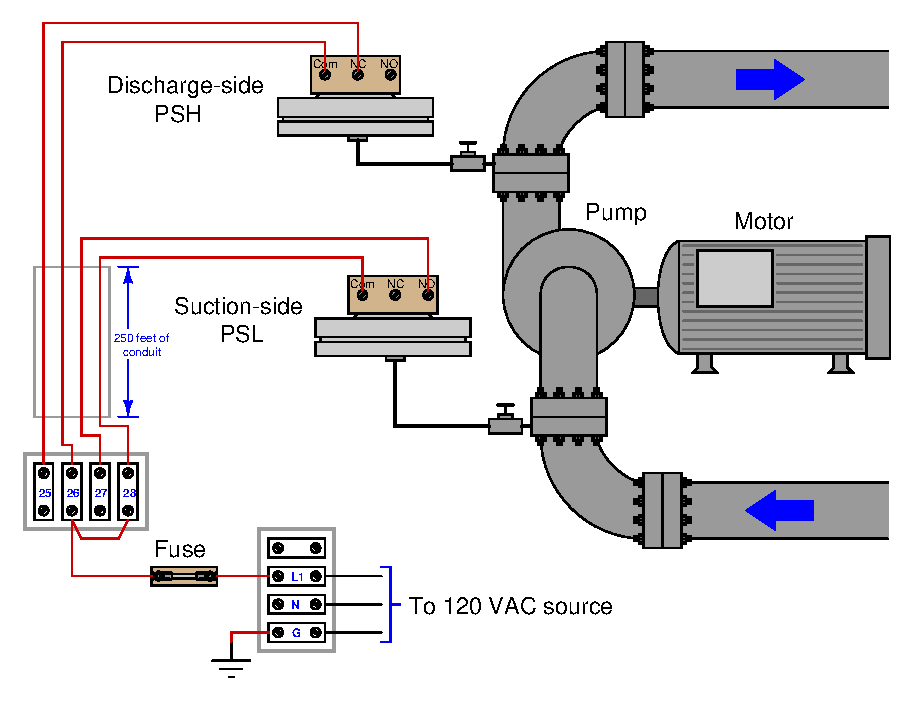
\includegraphics[width=15.5cm]{i02542x01.eps}$$

Using a digital multimeter (DMM), the technician first measures 118 VAC between terminals ``L1'' and ``N'' (to check the meter for proper operation).  Next, he measures 118 VAC as expected between terminal 25 and terminal ``N''.  For the last test, the technician measures 41 volts between terminal 27 and ``N''.  This last result was very unexpected!  Thinking perhaps the PSL switch is faulty, he walks to the field location and measures resistance between the ``Com'' and ``NO'' terminals on that switch, measuring infinite (``OL'') resistance with his multimeter.

\vskip 10pt

A fellow technician says to the first technician, ``Oh, that 41 volt measurement is just a {\it phantom voltage}.  Ignore it!''  Explain what this technician means by the phrase ``phantom voltage'' and comment on whether or not you think it should be ignored.

\vskip 20pt \vbox{\hrule \hbox{\strut \vrule{} {\bf Suggestions for Socratic discussion} \vrule} \hrule}

\begin{itemize}
\item{} Explain why these two pressure switches are wired as they are (PSH wired NC and PSL wired NO).  In each case, what will an improper pressure do to the status of each switch?
\item{} How could the DMM be altered so as to not be fooled by ``phantom'' voltages again?
\end{itemize}

\underbar{file i02542}
%(END_QUESTION)





%(BEGIN_ANSWER)

``Phantom'' AC voltage measurements are caused by capacitive coupling between adjacent wires, which along with the DMM's extremely large input impedance (millions of ohms) forms a voltage divider so that the meter will register a substantial fraction of the AC line voltage.

%(END_ANSWER)





%(BEGIN_NOTES)

In order to make a DMM ``fool-proof'' with regard to phantom voltages, one must decrease its input impedance.  Connecting a resistance (such as 20 k$\Omega$) across the input terminals of the voltmeter will load down any coupled signals, greatly reducing their magnitude.  Of course, the resistor must be appropriately sized such that the application of a ``real'' voltage of significant magnitude will not cause damage!

%INDEX% Electronics review: phantom AC voltage measurements
%INDEX% Switch, pressure: ``normal'' status of contacts

%(END_NOTES)


